\documentclass{beamer}

\usetheme{Darmstadt}

\usepackage{graphicx}
% \usepackage[utf8]{inputenc}
\usepackage[english]{babel}
\usepackage{amssymb,amsmath,mathtools}
\usepackage{amsfonts,amsthm} 
\usepackage{physics}
\usepackage[citestyle=verbose-ibid,, bibstyle=phys, biblabel=brackets, pageranges=true, backend=biber]{biblatex}
% \bibliography{source2.bib}
% \addbibresource{sources.bib}
\bibliography{sources2.bib}
\title{Topological phonons} 
\author{Christian Gommeringer}
\date{\today}

\def\hdis{\hspace*{-1cm}}

\begin{document}

% Title page frame\hdis
\begin{frame}
    \vspace{-0.2cm}\hdis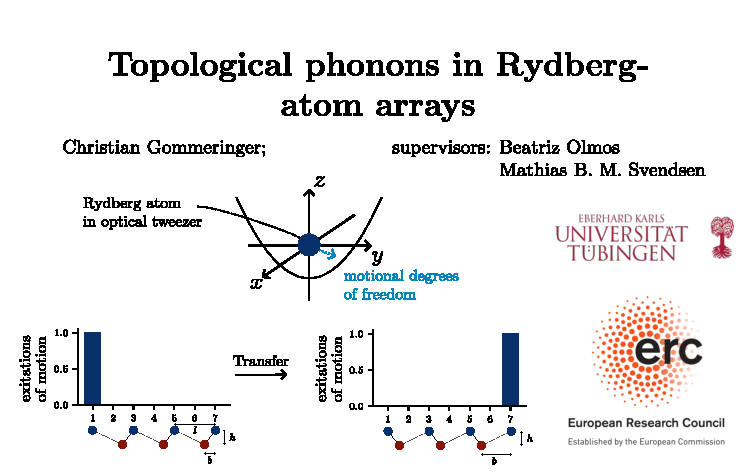
\includegraphics{presentation/title.pdf}
\end{frame}

% Remove logo from the next slides



% Outline frame
% \begin{frame}{Outline}
%     \tableofcontents
% \end{frame}

% \section*{topological phase}
% \begin{frame}{topological phase}
%     \textbf{symmetry protected topological states}\\
%     chiral symmetry implies form of Hamiltonian
%     \begin{align*}
%         \rightarrow H(\vec{k})=\begin{pmatrix}
%             0& h(\vec{k})\\
%             h^\dagger(\vec{k})&0
%         \end{pmatrix}
%     \end{align*}
% \end{frame}


\section*{SSH-model}
\begin{frame}{SSH-model}

    \vspace{-0.2cm}\hdis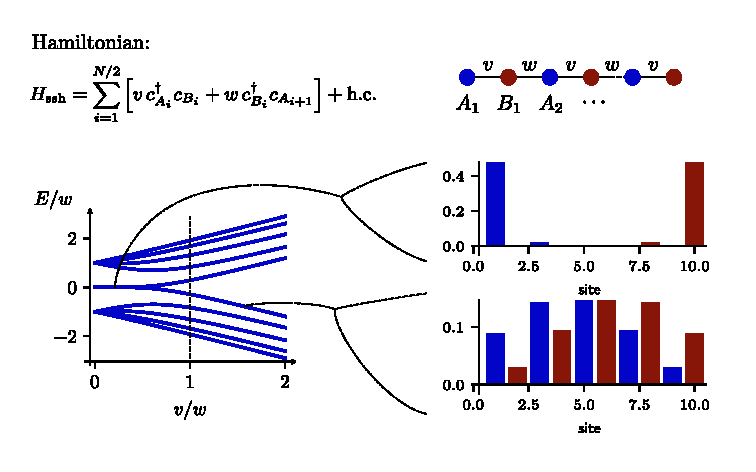
\includegraphics{presentation/ssh_model2.pdf}
\end{frame}


% \begin{frame}{Classification and robustness}

%     \vspace{-0.2cm}\hdis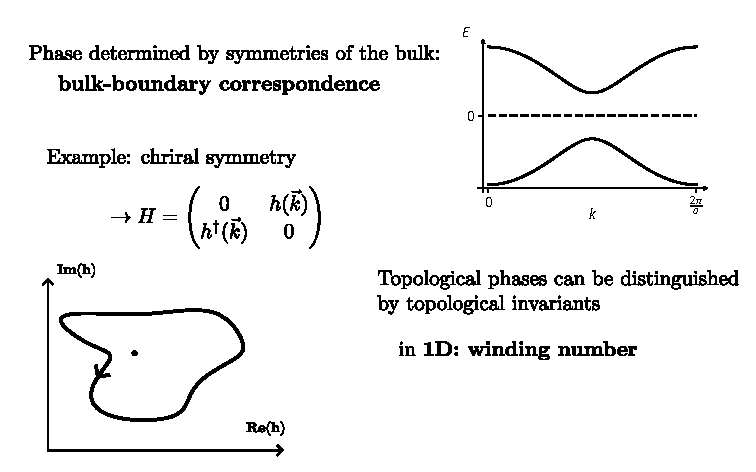
\includegraphics{presentation/Classification.pdf}
% \end{frame}


\section*{Model with Rydberg atoms}
\begin{frame}{Physical implementation}

    \vspace{-0.2cm}\hdis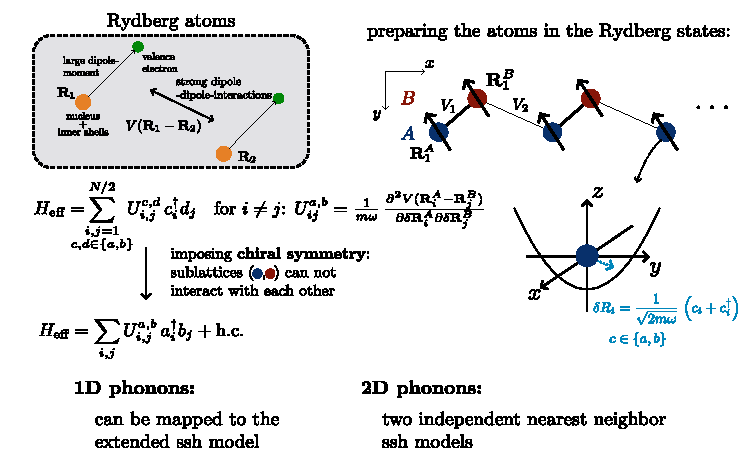
\includegraphics{presentation/slide_model2.pdf}
\end{frame}

\section*{Transfer}
\begin{frame}{Quantum state transfer}

    \vspace{-0.2cm}\hdis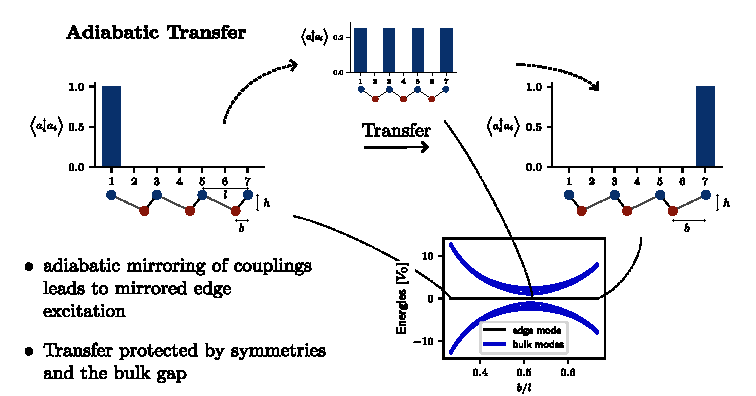
\includegraphics{presentation/slide_odd_transfer.pdf}
    \footnote{\cite{raupach_robust_2026}}
\end{frame}


% \begin{frame}{Transfer results}

%     \vspace{-0.2cm}\hdis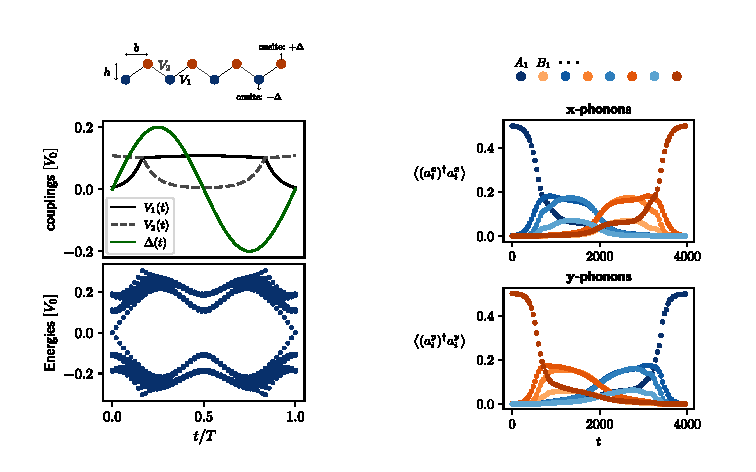
\includegraphics{presentation/results.pdf}
% \end{frame}

\section*{Outlook}
\begin{frame}{Summary and Outlook}

    \vspace{-0.2cm}\hdis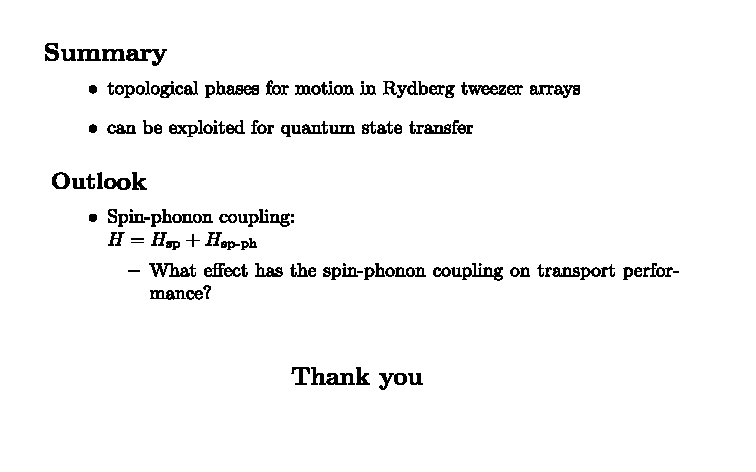
\includegraphics{presentation/outlook1.pdf}
\end{frame}


\end{document}